\documentclass{beamer}
\usepackage[latin1]{inputenc}
\usepackage{times}
\usepackage{tikz}
\usetheme{Luebeck}
%\usecolortheme{albatross}
\usepackage{amsmath,amsfonts,amsthm,amssymb}
\usepackage{setspace}
\usepackage{Tabbing}
\usepackage{fancyhdr}
\usepackage{lastpage}
\usepackage{extramarks}
\usepackage{chngpage}
\usepackage{soul,color}
\usepackage{graphicx,float,wrapfig}
\usepackage{xcolor}
\usepackage{listings}
\usepackage{float}
%\usepackage{subfloat}
\usepackage{subfigure}
\usepackage{caption}
\usepackage{enumitem}
\usepackage{algpseudocode}

\definecolor{darkorange}{RGB}{240, 120, 0}
\definecolor{darkgreen}{RGB}{0, 128, 0}
\definecolor{darkred}{RGB}{128, 0, 0}

\setbeamercolor{background canvas}{bg=white}
\setbeamercolor{frametitle}{fg=white, bg=darkorange}
\setbeamercolor{normal text}{bg=black,fg=black}
\setbeamercolor{structure}{bg=black, fg=darkorange}


\lstdefinestyle{customc}{
  belowcaptionskip=1\baselineskip,
  breaklines=true,
  frame=L,
  xleftmargin=\parindent,
  language=Python,
  showstringspaces=false,
  basicstyle=\footnotesize\ttfamily,
  keywordstyle=\bfseries\color{green!40!black},
  commentstyle=\itshape\color{purple!40!black},
  identifierstyle=\color{blue},
  stringstyle=\color{orange},
}

\lstdefinestyle{customc}{
  belowcaptionskip=1\baselineskip,
  breaklines=true,
  frame=L,
  xleftmargin=\parindent,
  language=Python,
  showstringspaces=false,
  basicstyle=\footnotesize\ttfamily,
  keywordstyle=\bfseries\color{green!40!black},
  commentstyle=\itshape\color{purple!40!black},
  identifierstyle=\color{blue},
  stringstyle=\color{orange},
}

\lstdefinestyle{customcsmall}{
  belowcaptionskip=1\baselineskip,
  breaklines=true,
  frame=L,
  xleftmargin=\parindent,
  language=Python,
  showstringspaces=false,
  basicstyle=\footnotesize\ttfamily,
  keywordstyle=\bfseries\color{green!24!black},
  commentstyle=\itshape\color{purple!24!black},
  identifierstyle=\color{blue},
  stringstyle=\color{orange},
}

\lstdefinestyle{customcsmall}{
  belowcaptionskip=1\baselineskip,
  breaklines=true,
  frame=L,
  xleftmargin=\parindent,
  language=Python,
  showstringspaces=false,
  basicstyle=\footnotesize\ttfamily,
  keywordstyle=\bfseries\color{green!24!black},
  commentstyle=\itshape\color{purple!24!black},
  identifierstyle=\color{blue},
  stringstyle=\color{orange},
}

\definecolor{MidGreen}{HTML}{00AA00}
\definecolor{MidYellow}{HTML}{AAAA00}

\title{Lecture 24: Heat Flow}
\date{4/12/2016}
\institute{Chris Tralie, Duke University}
\author{COMPSCI/MATH 290-04}
\begin{document}

\frame{\titlepage}

\begin{frame}{Announcements}
\begin{itemize}[label=$\vartriangleright$]

\item Group Assignment 3 Out: First Deadline Monday 4/18.  Final Deadline Wednesday 4/27 (Sakai says 4/26 but that's wrong...e-mail me solution if go until 4/27)

\item Final Project Final Deadline 5/3 5:00 PM

\end{itemize}

\end{frame}

\begin{frame}{Table of Contents}

\begin{itemize}[label=$\blacktriangleright$]
	\item Group Assignment 3 Preview
\end{itemize}

\begin{itemize}[label=$\vartriangleright$]
	\item Scalar Fields / Laplacian Review
\end{itemize}

\begin{itemize}[label=$\vartriangleright$]
	\item Heat Flow
\end{itemize}

\end{frame}


\begin{frame}{Group Assignment 3 Preview}
\begin{figure}[t]
    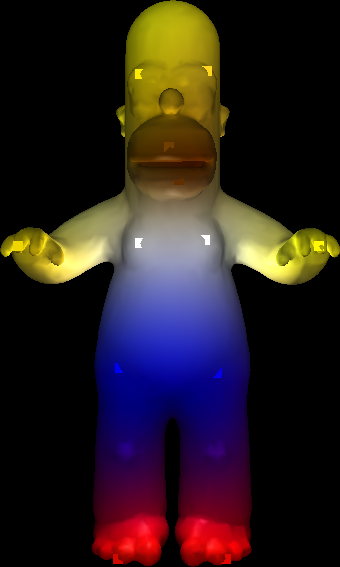
\includegraphics[width=0.4\textwidth]{ColorSolution.png}
\end{figure}

\end{frame}


\begin{frame}{Table of Contents}

\begin{itemize}[label=$\vartriangleright$]
	\item Group Assignment 3 Preview
\end{itemize}

\begin{itemize}[label=$\blacktriangleright$]
	\item Scalar Fields / Laplacian Review
\end{itemize}

\begin{itemize}[label=$\vartriangleright$]
	\item Heat Flow
\end{itemize}

\end{frame}


\begin{frame}{Mesh Scalar Fields (Functions)}

\begin{figure}[t]
    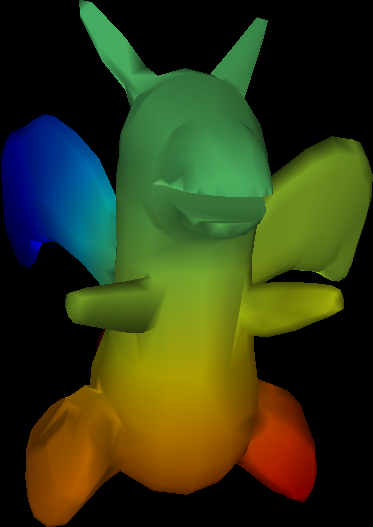
\includegraphics[width=0.4\textwidth]{DragonFunction.png}
\end{figure}

\begin{itemize}[label=$\vartriangleright$]
\item A real number for every point on the surface
\end{itemize}

\end{frame}

\begin{frame}{Coordinates As Functions}

\begin{figure}[t]
    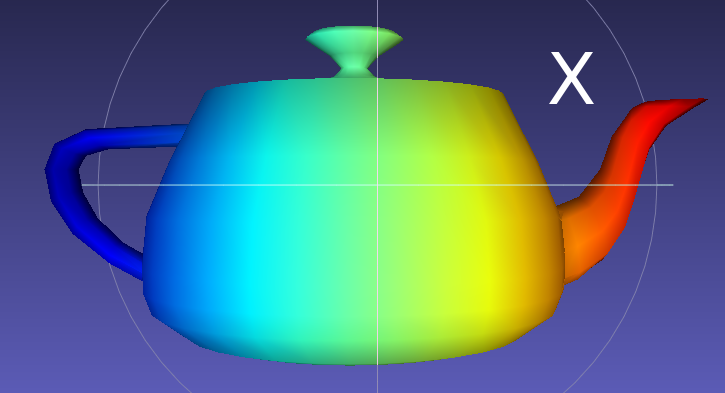
\includegraphics[width=0.4\textwidth]{TeapotX.png}
\end{figure}

\begin{figure}[t]
    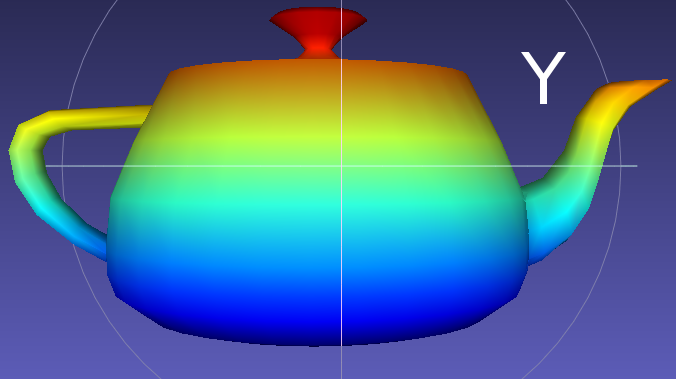
\includegraphics[width=0.4\textwidth]{TeapotY.png}
\end{figure}

\begin{figure}[t]
    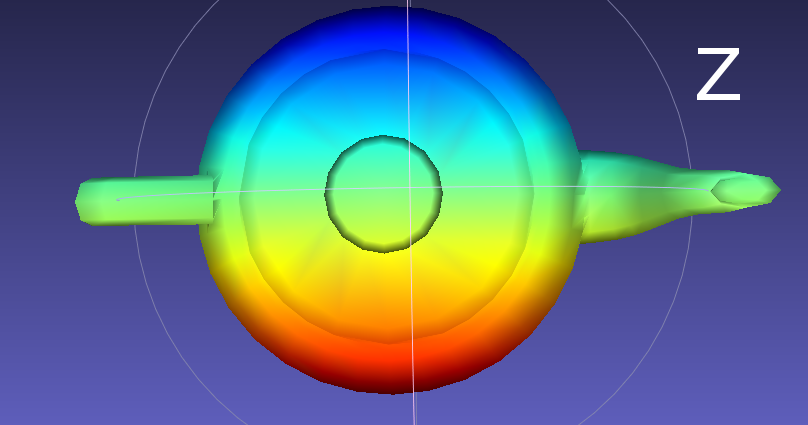
\includegraphics[width=0.4\textwidth]{TeapotZ.png}
\end{figure}
\end{frame}


\begin{frame}{Laplacian Eigenfunctions (Homer Modes)}

\[ L f = \lambda f \]

\begin{columns}
\begin{column}[T]{3cm}
\begin{figure}[t]
    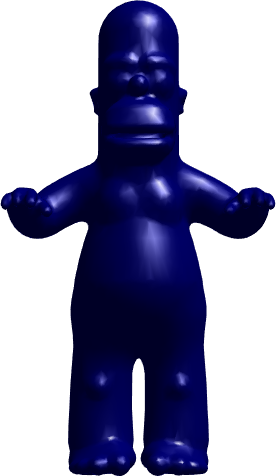
\includegraphics[width=\textwidth]{../23_Spectral/Harmonics/HomerModes/0.png}
    \caption*{\huge 0}
\end{figure}
\end{column}
\begin{column}[T]{3cm}
\begin{figure}[t]
    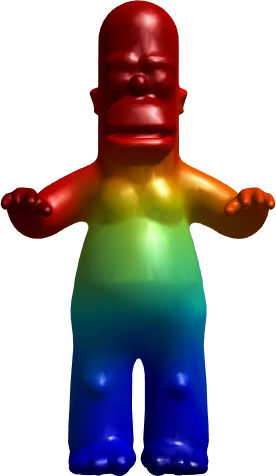
\includegraphics[width=\textwidth]{../23_Spectral/Harmonics/HomerModes/1.png}
    \caption*{\huge 1}
\end{figure}
\end{column}
\begin{column}[T]{3cm}
\begin{figure}[t]
    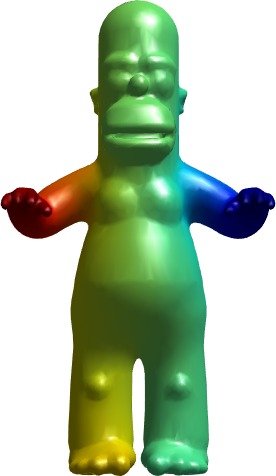
\includegraphics[width=\textwidth]{../23_Spectral/Harmonics/HomerModes/2.png}
    \caption*{\huge 2}
\end{figure}
\end{column}
\end{columns}

\end{frame}

\begin{frame}{Discrete Circle Laplacian Eigenvectors}

\begin{figure}[t]
    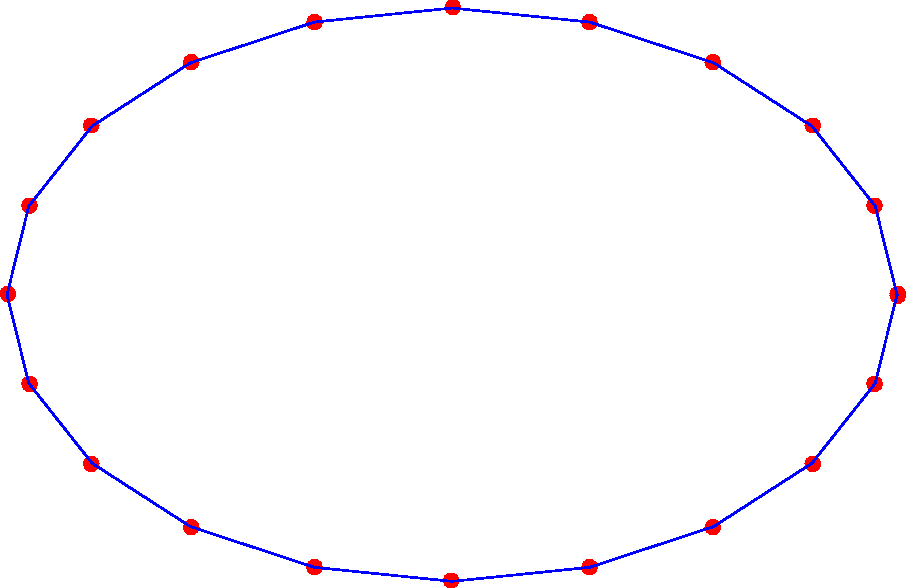
\includegraphics[width=0.32\textwidth]{CircleGraph.pdf}
\end{figure}

\begin{columns}
\begin{column}[T]{5cm}
\begin{figure}[t]
    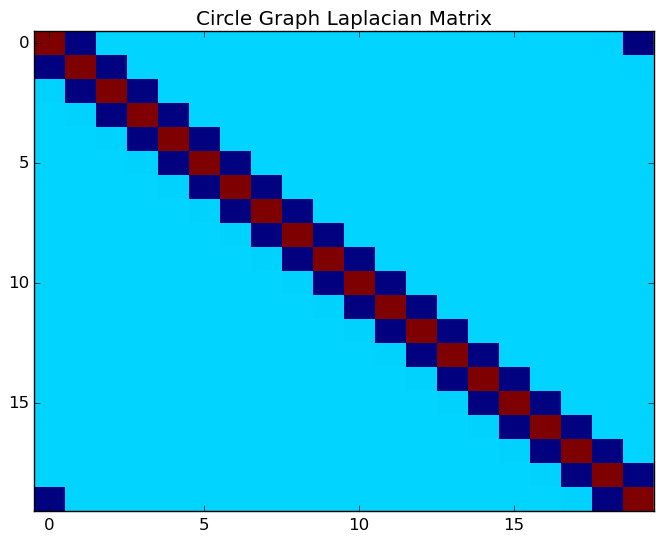
\includegraphics[width=\textwidth]{CircleLaplacian.png}
\end{figure}
\end{column}
\begin{column}[T]{5cm}
\begin{figure}[t]
    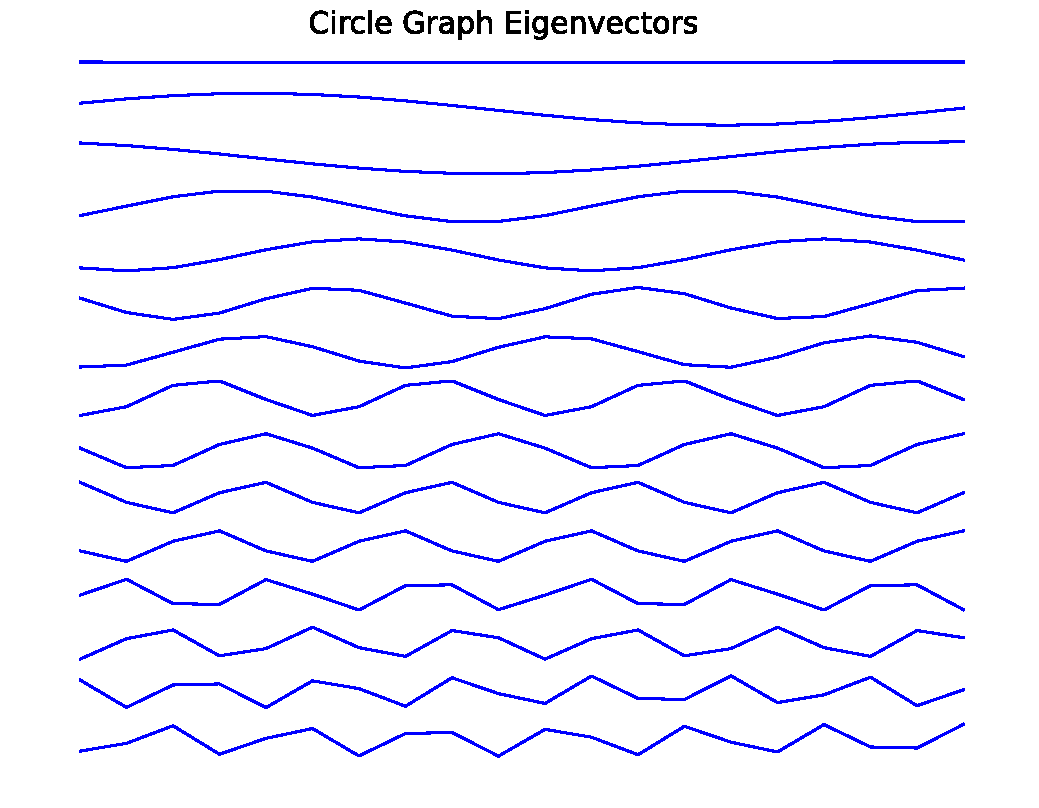
\includegraphics[width=\textwidth]{CircleEigvecs.pdf}
\end{figure}
\end{column}
\end{columns}

\tiny \url{https://github.com/COMPSCI290-S2016/NumpyDemos/blob/master/1DLaplacian.py}
\end{frame}

\begin{frame}{Discrete Circle Laplacian Eigenvectors}

\begin{figure}[t]
    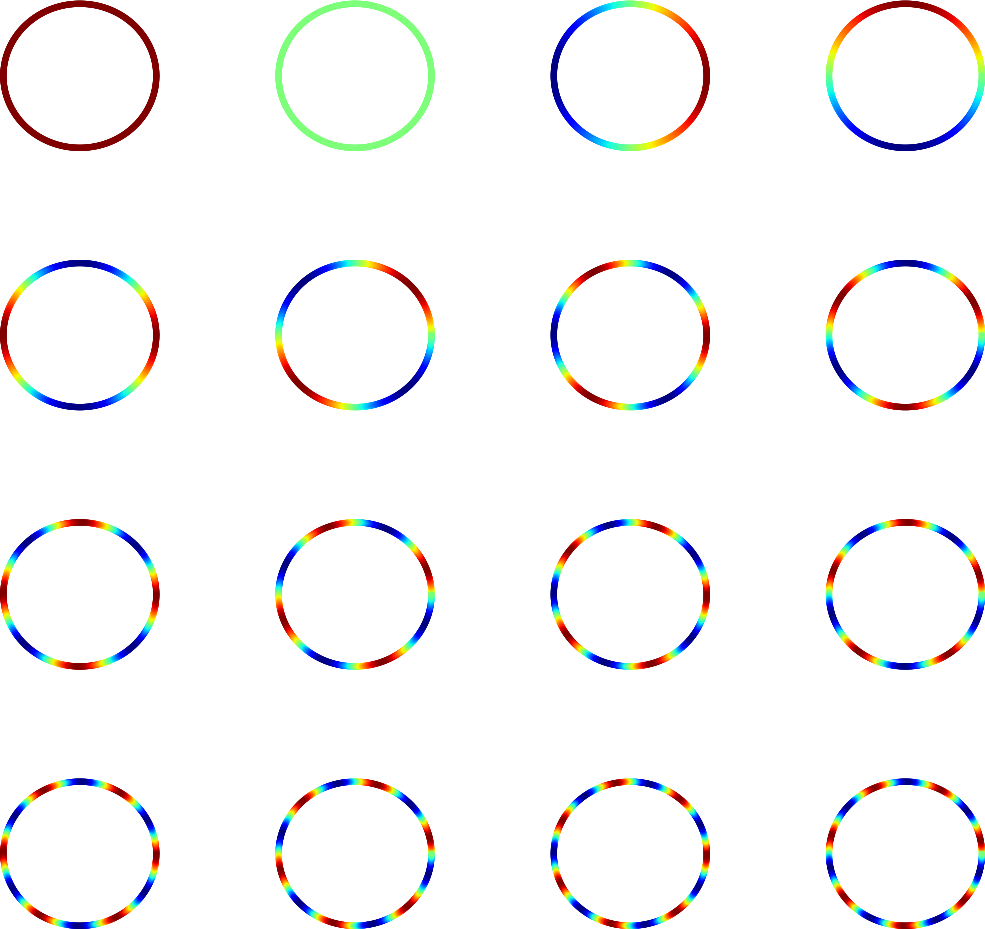
\includegraphics[width=\textwidth]{CircleFunctions.png}
\end{figure}

\end{frame}

\begin{frame}{Curvature Vector}

\[ \delta_x = Lx, \delta_y = Ly, \delta_z = Lz \]

\[ \delta = \sum_{j \in N(i)} (x_i, y_i, z_i) - (x_j, y_j, z_j) \]

\begin{figure}[t]
    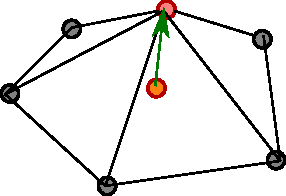
\includegraphics[width=0.5\textwidth]{2DDiscreteCurvature.pdf}
\end{figure}


\end{frame}

\begin{frame}{Table of Contents}

\begin{itemize}[label=$\vartriangleright$]
	\item Group Assignment 3 Preview
\end{itemize}

\begin{itemize}[label=$\vartriangleright$]
	\item Scalar Fields / Laplacian Review
\end{itemize}

\begin{itemize}[label=$\blacktriangleright$]
	\item Heat Flow
\end{itemize}

\end{frame}

\begin{frame}{1D Heat Equation}

Let $f(x, t)$ be the distribution of heat over a 1D bar of uniform material parameterized by $x$ at time $t$.  Then heat flow is governed by

\[ \frac{ \partial^2 f(x, t) }{ \partial x^2} = \frac{ \partial f(x, t) }{ \partial t} \]

\uncover<2->{

\begin{itemize}[label=$\vartriangleright$]
\item The higher the curvature of the heat distribution, the faster it dissipates
\end{itemize}

}

\end{frame}

\begin{frame}{1D Heat Flow Example}

\begin{figure}[t]
    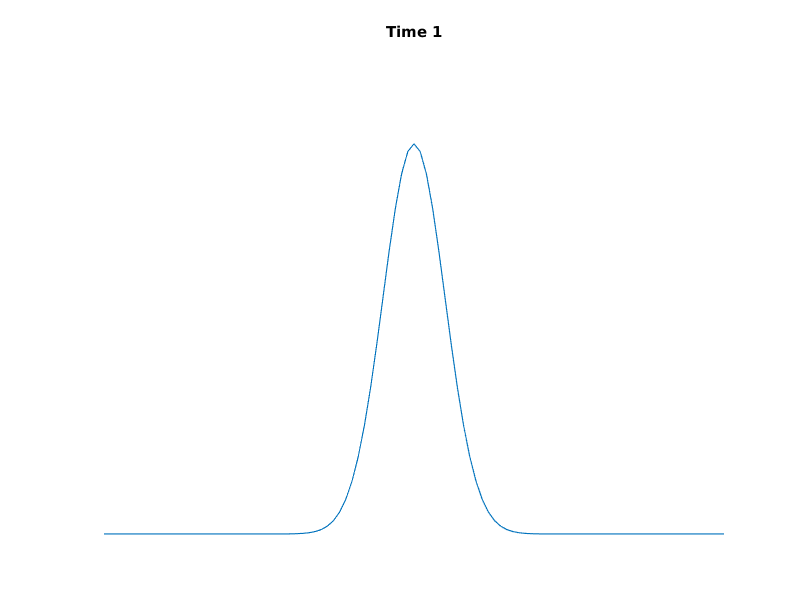
\includegraphics[width=\textwidth]{1.png}
\end{figure}

\end{frame}

\begin{frame}{1D Heat Flow Example}

\begin{figure}[t]
    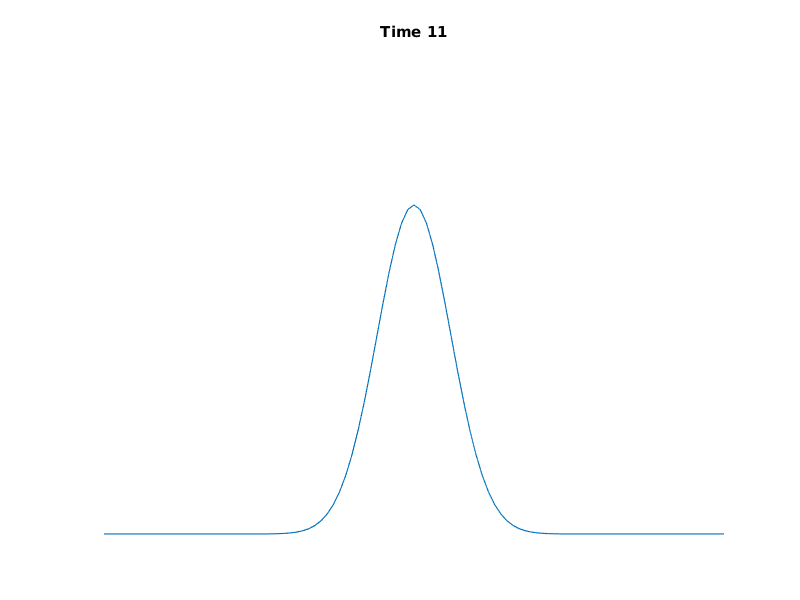
\includegraphics[width=\textwidth]{2.png}
\end{figure}

\end{frame}

\begin{frame}{1D Heat Flow Example}

\begin{figure}[t]
    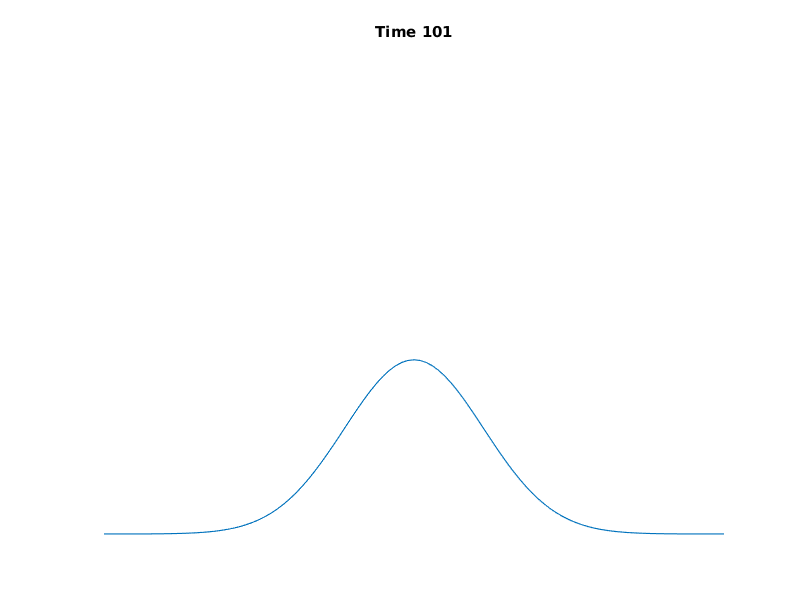
\includegraphics[width=\textwidth]{3.png}
\end{figure}

\end{frame}

\begin{frame}{1D Heat Flow Example}

\begin{figure}[t]
    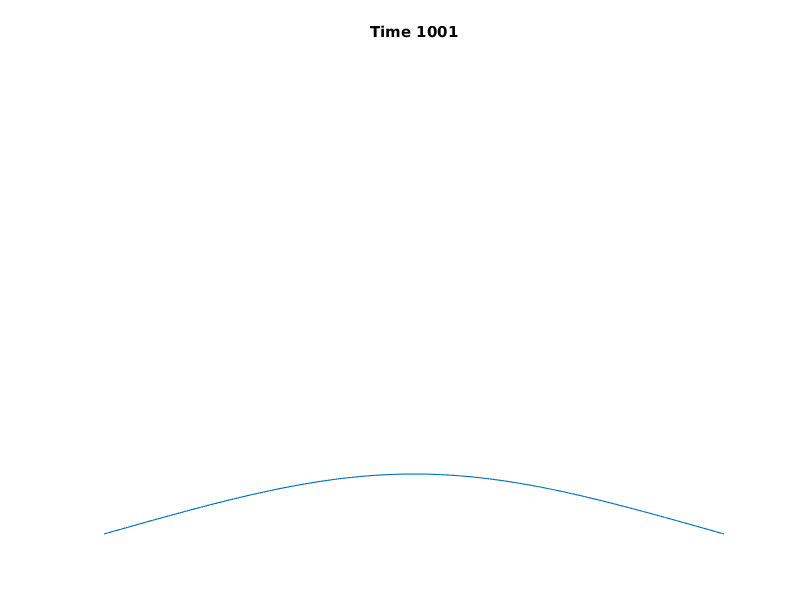
\includegraphics[width=\textwidth]{4.png}
\end{figure}

\end{frame}

\begin{frame}{1D Heat Flow Example}

\begin{figure}[t]
    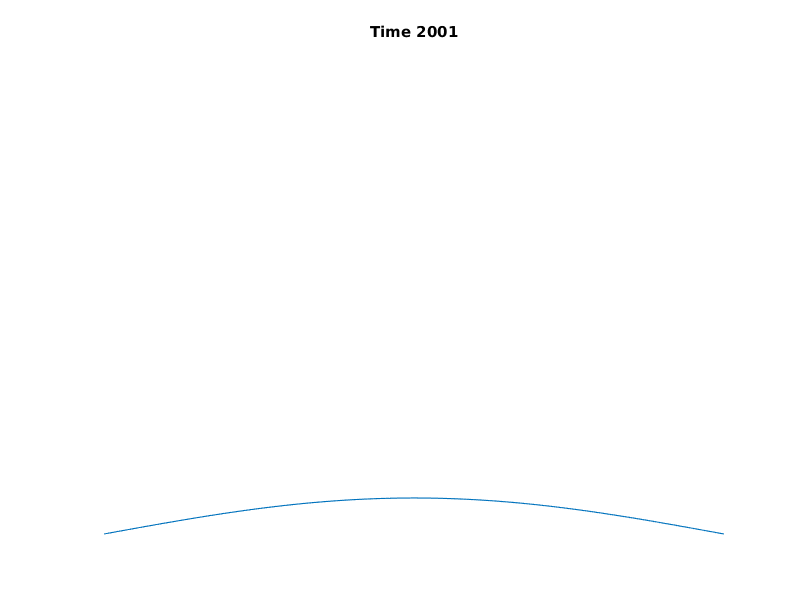
\includegraphics[width=\textwidth]{5.png}
\end{figure}

\end{frame}


\begin{frame}{Generalizing To Surfaces}

\[ \frac{ \partial^2 f(x, t) }{ \partial x^2} = \frac{ \partial f(x, t) }{ \partial t} \]

Let $f$ be the discrete values of a function on a mesh.  What is the heat equation?

\uncover<2->{
\[ Lf = -\frac{ \partial f}{\partial t} \]
}

\uncover<3->{
Video example...
}

\end{frame}

\begin{frame}{Solutions To The Heat Equation}

\[ \frac{ \partial^2 f(x, t) }{ \partial x^2} = \frac{ \partial f(x, t) }{ \partial t} \]

\uncover<2->{
\[ f_{\omega} = \cos(\omega x) e^{-\omega^2 t} \]
}

\uncover<3->{
\[ Lf = -\frac{ \partial f}{\partial t} \]
}

\uncover<4->{
Let $\phi_k$ be the $k^\text{th}$ eigenvector of $L$ and $\lambda_k$ be the associated eigenvalue.  Then solutions are

\[ f_k = \phi_k e^{- \lambda t} \]

}

\end{frame}

\begin{frame}{Initial Conditions}

What if initial condition $f_0$ doesn't happen to be an eigenvector of $L$?

\uncover<2->{

\begin{itemize}[label=$\vartriangleright$]
\item Project $f_0$ onto eigen basis, sum the solutions of each eigenvector individually

\[ f(t) = \sum_k (f_0^T \phi_k) e^{-\lambda_k t} \phi_k \]

\end{itemize}

}

\uncover<3->{
Demo...
}

\end{frame}


\begin{frame}{Heat Kernel Signature}
For every point, the fraction of heat that stays at that point after a certain amount of time


\begin{minipage}{0.45\textwidth}{
$t = 20$
\begin{figure}[t]
    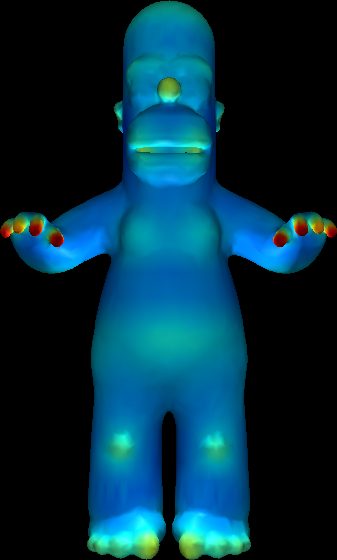
\includegraphics[width=0.6\textwidth]{HomerHKS_20.png}
\end{figure}
}
\end{minipage}
\begin{minipage}{0.45\textwidth}
$t = 500$
\begin{figure}[t]
    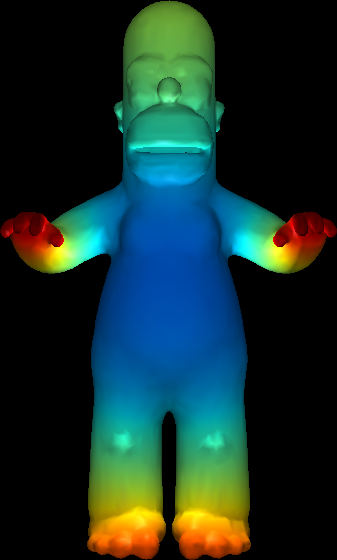
\includegraphics[width=0.6\textwidth]{HomerHKS_500.png}
\end{figure}
\end{minipage} \\


What does this look like? \uncover<2->{ \textcolor{red}{Multiscale curvature} }

\end{frame}

\begin{frame}{Heat Kernel Signature: Computations}

\[ f(t)[i] = \sum_k (f_0^T \phi_k)[i] e^{-\lambda_k t} \phi_k[i] \]

\uncover<2->{
By definition, starting with a unit amount of heat at every point
\[ f_0[a] = \left\{ \begin{array}{cc} 1 & a = i \\ 0 & \text{otherwise} \end{array} \right\} \]
}


\uncover<3->{
\[ f(t)[i] = \sum_k \phi_k[i] e^{-\lambda_k t} \phi_k[i] \]


\[ f(t)[i] = \sum_k e^{-\lambda_k t} \phi_k[i]^2 \]

}

\end{frame}

\begin{frame}{Another Example}

\begin{minipage}{0.45\textwidth}{
$t = 20$
\begin{figure}[t]
    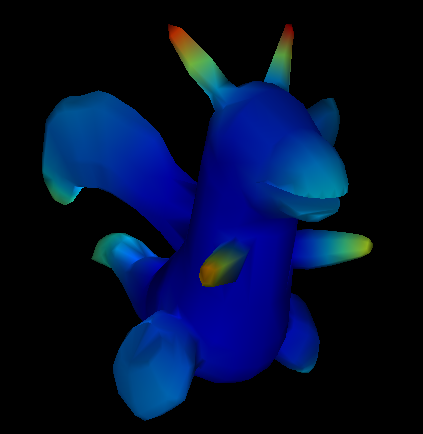
\includegraphics[width=0.8\textwidth]{DragonHKS_20.png}
\end{figure}
}
\end{minipage}
\begin{minipage}{0.45\textwidth}
$t = 500$
\begin{figure}[t]
    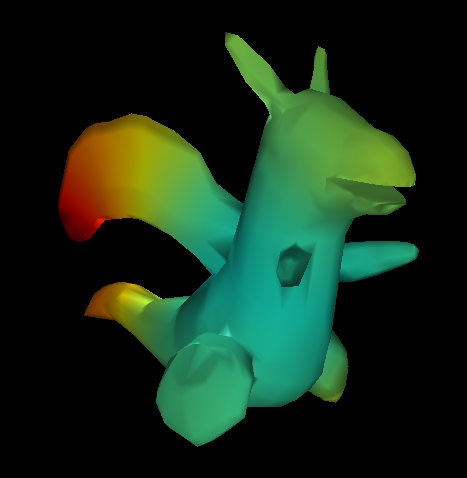
\includegraphics[width=0.8\textwidth]{DragonHKS_200.png}
\end{figure}
\end{minipage}

\end{frame}

\end{document}

